\section{Architecture}
%
This section introduces the architecture of the current version of PostgreSQL.
%
Furthermore it is shown how the architecture looks after the refactoring and implementation of the new algorithm.
%
\subsection{Current architecture}
%
In the current version of PostgreSQL the access control module is not identifiable as a stand-alone module in the backend code of the DBMS.
%
Figure~\ref{figure:postgresql:architecture} shows a flowchart of a PostgreSQL server instance.
%
The flowchart shows backend's behaviour.
%
\subsubsection{Backend architecture}
%
Each box in the flowchart represents a module of PostgreSQL.

The \emph{Main} module is responsible for checking the underlying system requirements, i.e., the system user starting the server, available memory etc. If all the requirements are met the \emph{Postmaster} process is started.

The Postmaster is the starting point for any PostgreSQL server instance. 
%
In this module system setup tasks such as loading the data representing the database and setting up listeners for database connections are executed.
%
After setting everything up the Postmaster waits for a connection request from a \emph{frontend application}, which refers to any application that connects to the database.
%
When receiving a connection request the Postmaster forks itself.
%
The child process then will either authorize the request and become a \emph{Backend} or reject the request and exit.
%
All the blue boxes in the flowchart represent modules of the Backend of a PostgreSQL server.

The Backend consists of an infinite loop which breaks at the parser stage.
%
At this point the Backend is ready to receive a query from the connected frontend application.
%
After receiving a query in text form the parser creates the abstract syntax tree representing the query.
%
The abstract syntax tree is then passed to the \emph{Traffic Cop}.

The Traffic Cop first analyzes the query to classify it either as a \emph{utility query} or \emph{non-utility query}.
%
Utility queries modify the structure of the databse, e.g., create/drop a table, create/drop a view, create/drop a trigger etc.
%
Non-utility queries act on the data inside the database, e.g., select tuples, insert tuples, update tuples etc.
%
After determining the type the Traffic Cop forwards utility queries to the \emph{Utility Command} module, which will check the authorization of the query and, if the query is authorized, execute it.
%
Non-utility commands are forwarded to the \emph{Rewrite Query} module.

Here the query is rewritten according to the \emph{PostgreSQL Rule System}, which is a collection of rules on how to rewrite queries, such that they are optimized for PostgreSQL.
%
After that the rewritten query is passed to the \emph{Generate Paths} module.
%
Here the system generates different \emph{paths} to execute the query.
%
Each path represents a way of executing the query, i.e., a possible way of traversing the abstract syntax tree.
%
According to internal rules the system will choose the optimal path.
%
This path is passed to the \emph{Generate Plan} module, which internally will generate a \emph{plan} for the executor.
%
A plan is detailed guide for the executor on how to retrieve the tuples.

This plan is then forwarded to the executor, which will execute it and return the tuples to the frontend application.
%
\begin{figure}[!ht]
  \centering
    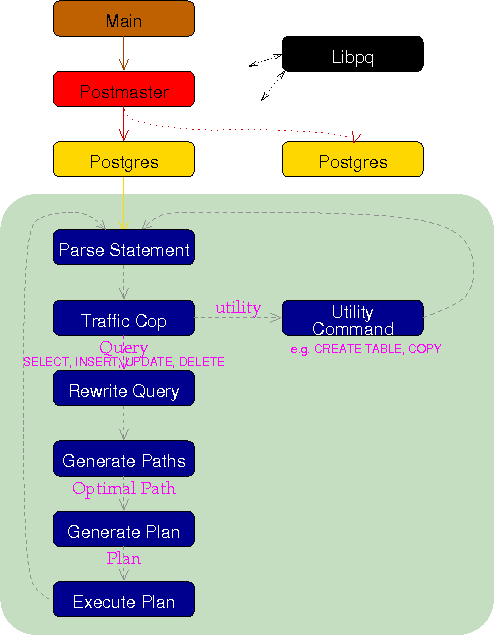
\includegraphics[width=1\textwidth]{img/backend_flowchart.png}
    \caption{Backend Flowchart PostgreSQL \protect \footnotemark}\label{figure:postgresql:architecture}
\end{figure}
%
\footnotetext{\url{http://www.postgresql.org/developer/backend}}
%
\FloatBarrier
\subsubsection{Access Control}
%
Access control decisions can be made in any of the the following: Traffic cop, Executor, or in the module that handles the utility queries.
%
The functions making these decisions, however also prepare the system for the upcoming change, by, e.g., returning address where a new table is allocated.
%
Due to the distribution and inconsistency of the access control mechanism, there is no uniform interface that can be called for such a decision.
%
Furthermore  the mechanism is, at some points, closely connected to the internals of the database, making the implementation of a new mechanism nearly impossible without refactoring the code.
%
\subsection{Refactoring}
%
After analyzing the backend, by executing each type of query and following the backend throught the process with a debugger, all the functions or code regions relevant to making access control decisions was identified.
%
This identification allowed to gradually move the code to an external module and build a uniform interface which is called inside the traffic cop, when the backend expects a decision. 
%
The building of a uniform interface however introduced several engineering challenges.
%
The first decision was to create a stand-alone module in the backend of PostgreSQL, which allows developers to clearly identify the code that is responsible for authorizing any type of query.
%
Second we built an interface, that can be called from any module, when requiring an access control decision.

The interface looks as follows:
%
\begin{lstlisting}[frame=single, style=customc]
ac_return_data authorized(ac_decision_data *decision_data);
\end{lstlisting}
%
The structs used in the interface are extensible. For each type of query there is a field in both structs, which represent the input and output data for the all queries of this type.
%
The structs look as follows:
\begin{lstlisting}[frame=single, style=customc]
union ac_return_data_struct {
	Oid target_namespace; /* Returned if CREATE is authorized */
	AclMode current_privileges; /* Returned if GRANT is authorized */
	bool execute; /* Returned for Non-utility query */
};

struct ac_decision_data_struct {
	command_type command;
	ac_create_relation_data *create_relation_data; /* If (command == CREATE_RELATION) this cannot be NULL */
	ac_grant_data *grant_data; /* If (command == GRANT || command == REVOKE) this cannot be NULL */
	ac_nutility_data *nutility_data; /* If (command == INSERT || command == DELETE || command == SELECT) this cannot be NULL */
	ac_create_trigger_data *create_trigger_data; /* If (command == CREATE_TRIGGER) this cannot be NULL */
};
\end{lstlisting}
%
Further each field in the decision data struct is actually a pointer that refers to a struct, that in turn holds all information needed for deciding if the respective type of query is authorized.
%
Any function that calls this interface will pass all the data needed to make the decision.
%
Depending on the data received the interface internally calls the functions that were previously distributed among the modules.
%
This allows for future developers to gradually implement a new algorithm, by identifying the query received, and either return the result of a new algorithm, or call the original function responsible for the query.
%
To facilitate the identification of the query received we have included an additional field in the decision data, which tells exactly what type of query was received by the interface, i.e., \texttt{INSERT} or \texttt{UPDATE} instead of just identifying it as a non-utility query.
%
Further we added a stack that at any point of the execution of the database system, holds all queries that are not yet completed.
%
This allows developers to always have a clear view on the state of the database system.
%
The stack is used to simplify the implementation of novel mechanisms such as the one in~\cite{guarnieri2016strong}, since the algorithm from Guarnieri et. al requires knowledge about other aspects of the system such as triggers being executed, or nested queries.
%
After the process of refactoring it is possible to integrate any access control mechanism as a plug-in.